%; whizzy chapter
% -initex iniptex -latex platex -format platex -bibtex jbibtex -fmt fmt
% 以上 whizzytex を使用する場合の設定。

%     Tokyo Debian Meeting resources
%     Copyright (C) 2011 Junichi Uekawa
%     Copyright (C) 2011 Nobuhiro Iwamatsu

%     This program is free software; you can redistribute it and/or modify
%     it under the terms of the GNU General Public License as published by
%     the Free Software Foundation; either version 2 of the License, or
%     (at your option) any later version.

%     This program is distributed in the hope that it will be useful,
%     but WITHOUT ANY WARRANTY; without even the implied warranty of
%     MERCHANTABILITY or FITNESS FOR A PARTICULAR PURPOSE.  See the
%     GNU General Public License for more details.

%     You should have received a copy of the GNU General Public License
%     along with this program; if not, write to the Free Software
%     Foundation, Inc., 51 Franklin St, Fifth Floor, Boston, MA  02110-1301 USA

%  preview (shell-command (concat "evince " (replace-regexp-in-string "tex$" "pdf"(buffer-file-name)) "&"))
% 画像ファイルを処理するためにはebbを利用してboundingboxを作成。
%(shell-command "cd image201201; ebb *.png")

%%ここからヘッダ開始。

\documentclass[mingoth,a4paper]{jsarticle}
\usepackage{monthlyreport}

\begin{document}

\dancersection{Rabbit: 時間内に終われるプレゼンツール}{須藤功平}
\label{sec:kou}

Debian GNU/Linux上で動作するプレゼンテーションツールRabbitを紹介します。

Debian GNU/Linux上で動作するプレゼンテーションツールはたくさんあります。

\begin{itemize}
 \item LibreOfficeのImpress
 \item LaTeXのBeamerクラス + PDFビューアー(Evinceやpdfcubeなど)
 \item JavaScript + Webブラウザ(Impress.jsやshowoffなど)
 \item Webサービス(Google DocsやPreziなど)
 \item MagicPoint
 \item Rabbit
\end{itemize}

それぞれのツールは特徴が大きく異なっており、それぞれよいところがありま
す。Rabbitにもまた特徴があり、他のツールにはない便利な機能があります。
それが「プレゼンテーションを時間内に終わらせるための機能」です。プレゼ
ンテーション中に残り時間を表示して、発表者に進み具合を伝えるタイマー機
能は多くのツールが提供しています。Rabbitの機能はどう違うのでしょうか。
一言でいうとUI(ユーザーインターフェイス。見た目)が違います。他は同じ
です。

\subsection{RabbitのUI}

タイマー機能はMagicPointも提供していますし、Impressも提供しています。
図\ref{fig:normal-timer-ui}のように、MagicPointはスライド下部にとても目
立たないように緑のバーを表示します。Impressはスライド表示用のモニターと
は別のモニターに経過時間を表示します。このように発表者にだけわかるよう
に表示するUIが一般的なタイマー機能のUIです。

\begin{figure}[ht]
  \begin{center}
    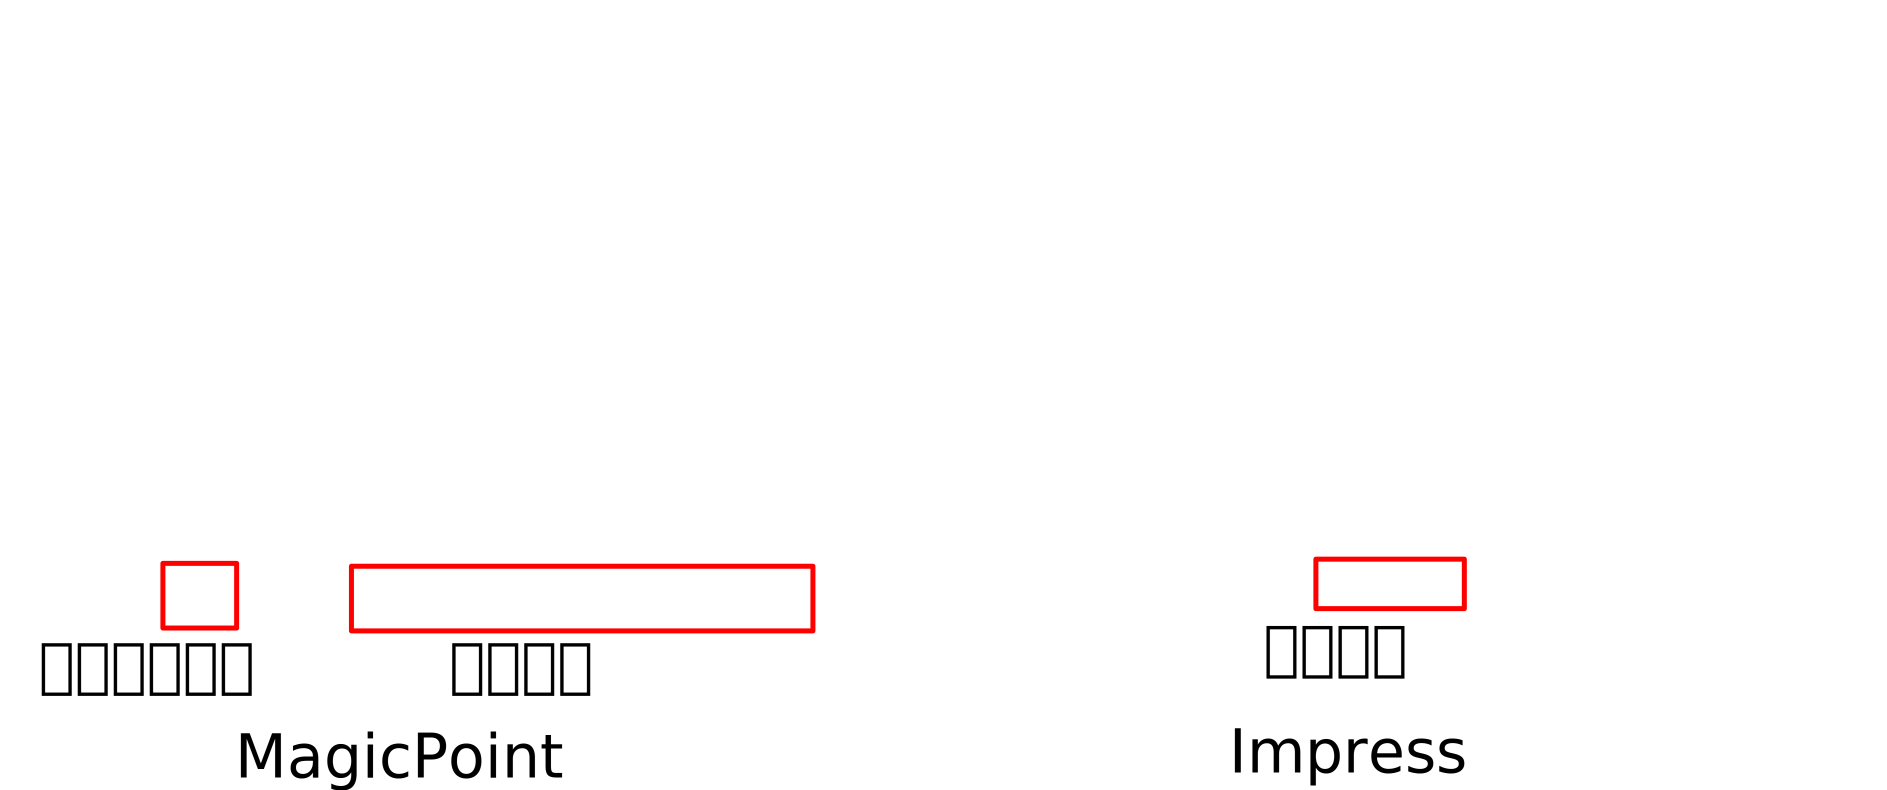
\includegraphics[width=1\hsize]{images/normal-timer-ui.eps}
  \end{center}
  \caption{従来のタイマー機能のUI}
  \label{fig:normal-timer-ui}
\end{figure}

一方、RabbitのUIは発表者だけではなく観客にもわかりやすく表示します。
図\ref{fig:rabbit-timer-ui}のように、スライド下部にうさぎとかめを表示し
ます。それも誰が見ても気づくくらいの大きさで表示します。このようにタイ
マー機能を観客からもわかりやすく表示するUIは既存のプレゼンテーションツー
ルとは一線を画します。

\begin{figure}[ht]
  \begin{center}
    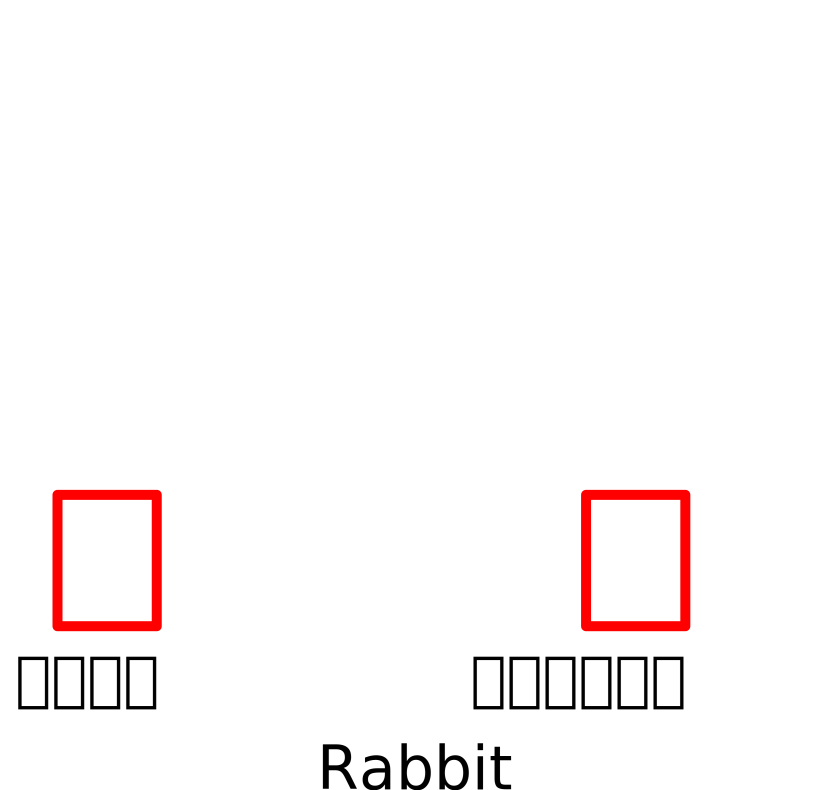
\includegraphics[width=0.5\hsize]{images/rabbit-timer-ui.eps}
  \end{center}
  \caption{Rabbitのタイマー機能のUI}
  \label{fig:rabbit-timer-ui}
\end{figure}

それでは、このUIがどうして時間内に終わるための効果を提供するかを考えて
みましょう。

\subsubsection{サブサブセクション}

サブサブセクション。

\begin{commandline}
コマンドラインとか。
% apt-get
\end{commandline}

フットノート\footnote{フットノートです。}

\begin{itemize}
\item リスト1
\item リスト2
\end{itemize}


\begin{enumerate}
\item 番号付きリスト1
\item 番号付きリスト2
\end{enumerate}

Debian GNU/Linuxでプレゼンテーションをする人たちの参考になることを期待
します。

\end{document}
